In this section we come up with some approaches on how to measure uniformity of prediction. The typical way of 'checking' uniformity of prediction used by physicists 
is fitting the distribution of the events that were classified as signal (or background) over the mass (or some other variable).

This approach is hardly formalizable, and not automatable --- each time you should assume some kind of distribution. 
Ideally we want to have some easy-to-use out-of-the-box metrics like FOMs in machine learning (like area under the ROC, f1 or ).

\subsection{Ideal uniformity}

We start from the simplest case --- when we are fully satisfied by predictions of our classifier. Remember that output of 
classification is probabilities of each event being a signal and background event, only after we select some cut on probability we get classification.

Ideal uniformity of signal prediction means that whichever cut we select, the efficiency (part of signal event that passed the cut) doesn't depend on uniform variables: 
in every region of uniform variables space the part of signal events that passed the cut is the same.

In practice, of course, this never happens.

There is uniformity of predictions on signal and uniformity of efficiency on background, which can be defined one from another by swapping classes. 
In what follows in this section we are writing about the efficiency on signal events.

A good example of classifier that has close to ideal uniformity is classifier which returns a random probability in [0, 1] range. What a pity: in practice it's absolutely useless.

% The most significant drawback of the upcoming metrics is they are ill-defined if there are not too many events of the named class. 

\subsection{Some Restrictions on Uniformity Metrics}

There are some additional conditions which we expect metric to meet:
\begin{enumerate}
\item
shouldn't depend much on the number of events (i.e., if we randomly select half of the events, the metrics should roughly be the same)
\item
shouldn't depend on the weights renormalization: if we multiply all the weight by some arbitrary number, it shouldn't change at all.
\item 
depends only on the order of predictions, not the exact values of probabilities.
This is because we care about which events pass the cut and which don't, not about the exact values of predictions.

Example: correlation of prediction and mass doesn't satisfy this restriction.
\item
parameter stability: if it uses bins, changing the number of bins shouldn't affect the metrics value much, if it uses $k$-nearest neighbors, it should be stable to small deviations of $k$.
\end{enumerate}


\subsection{Standard Deviation of Efficiency on Bins (SDE)}

\def\bineff{\text{eff}_\text{bin}}
\def\binweight{\text{weight}_\text{bin}}
\def\globaleff{\text{eff}}
\def\SDE{\text{SDE}}
\def\bin{\text{bin}}


Let's split the space of uniform features into bins, the uniformity in these terms is following: when we select some probability cut, 
the part of signal events that passes the cut is equal in all bins. Assume we selected some cut, then we have global efficiency
\[
	\globaleff = \dfrac{
		\text{total weight of signal events that passed the cut}}
		{\text{total weight of signal events}}
\]

Efficiency in every bin is defined respectively, 
\[
	\bineff = \dfrac{
		\text{weight of signal events in bin that passed the cut}}
		{\text{weight of signal events in this bin}} 
\]

So, basically, what we want to have in our dreams:
\[
	\bineff = \text{global efficiency} \qquad \forall \; \text{bin}
\]


To measure how far we are from ideal situation we use standard deviation:
\[
	\sqrt{\sum_{\bin} \left( \bineff - \globaleff \right)^2  }
\]

What is bad in this formula that every bin has some impact in the result, which does not depend on how many events are there, so metrics becomes very unstable to deviations in bins with only few events. To cure this, we add weights to the bins (note that $\sum_\bin \binweight = 1$):
\[
	\binweight = \dfrac{\text{total weight of signal events in bin}}
		{\text{total weight of signal events}},
\]
so we have SDE formula:
\[
	\SDE(\globaleff) = 
	\sqrt{\sum_{\bin} \binweight \times \left(\bineff - \globaleff \right)^2}. 
\] 
In fact, the expression depends on the cut, but for cuts which produce equal efficiency, this is 


Finally we note that the weighted average of $\bineff$ is $\globaleff$:
\[
	\globaleff = < \bineff > =  \sum_{\bin} \binweight \times \bineff,
\]
and this is why the introduced metrics was named SDE --- this is a weighted standard deviations of array of bin efficiencies.

But this is how we measure the non-uniformity for only one fixed cut, to measure the overall non-flatness, we take several global efficiencies (for instance, [0.5, 0.6, 0.7, 0.8, 0.9], because in practice usually we are interested in cuts with high global efficiency) and use 
\[
	\SDE^2  =  \frac{1}{k} 
	\sum_{\globaleff \in [\globaleff_1 \dots \globaleff_k] }  
		\text{SDE}^2(\globaleff)
\]

Some other power $p \neq 2$ can be used as well, but $p=2$ is considered as the default value: 
\[
	\SDE^p(\globaleff) = 
	\sum_{\bin} \binweight \times \abs{\bineff - \globaleff}^p,
\qquad
	\SDE^p  =  \frac{1}{k} 
	\sum_{\globaleff \in [\globaleff_1 \dots \globaleff_k] }  
		\text{SDE}^p(\globaleff).
\]



\subsection{Theil Index of Efficiency}
\def\theil{\text{Theil}}

One more measure uses Theil Index frequently used to measure economic inequality:
\[
	\theil = \frac{1}{N} \sum_i \frac{x_i}{<x>} \ln{\frac{x_i}{<x>}}, 
		\qquad <x> = \frac{1}{N} \sum_i x_i
\]
In our case we have to alter formula a bit to take into account that different bins have different impact, thus the formula turns into
\[
	\theil(\globaleff) = \sum_\bin \binweight \; \frac{\bineff}{\globaleff} \; \ln{\frac{\bineff}{\globaleff}}
\]

TODO how to combine Theil for different global efficiencies?
\[
	\theil = ??? \text{from} \theil(\globaleff)
\]

\subsection{Distribution Similarity Approach}
\label{sec:similarity}

Let's start from reformulation of what is uniform predictions in signal. First we split all signal events into some bins in uniform variables. There is some empirical distribution $F_\bin$ of predictions in each bin. Ideal uniformity means that all the distributions $F_\bin$ are equal and hence equal to the global distribution $F(x)$. 

To 'measure' non-flatness we can use some distribution distance, like Kolmogorov-Smirnov:
\[
	 \sum_{\bin} \binweight \max_x \abs{F_{\bin}(x) - F(x)},
\]
but Cram\'er--von Mises similarity is more informative (usually $p=2$ is used):
\[
	 \sum_{\bin} \binweight \int \abs{F_{\bin}(x) - F(x)}^p dF(x),
\]

The good point is we don't need to select some global efficiencies like in the other metrics.


\subsection{Connection Between SDE and Distribution Similarity Approach}

SDE and DSA based on Cram\'er--von Mises similarity can be shown to have connection.
Let's consider the SDE with global efficiencies $= [1/N, 2/N, \dots, N/N]$. In the limit $N \to \infty$
\[
	\lim_{N \to \infty} \SDE^2 = 
	\lim_{N \to \infty} \frac{1}{N} \sum_{\globaleff}\SDE^2(\globaleff) = 
	\int_0^1 \SDE^2(\globaleff) d\, \globaleff = 
	\int_0^1 \sum_{\bin} \binweight \abs{\bineff - \globaleff}^2 d\, \globaleff
\]

From the other side, we can write the expression for similarity-based measure (for $p=2$) 
\[
	\sum_{\bin} \binweight \int \abs{F_\text{bin}(x) - F(x)}^2 dF(x) =
	\int \sum_{\bin} \binweight \abs{F_\text{bin}(x) - F(x)}^2 dF(x) 
\] The hard thing now is to believe this is literally the same and these two expressions are equal.


\subsection{Knn-based modifications}

\def\knni{\text{knn}(i)}
\def\effknni{\text{eff}_{\knni}}
\def\weightknni{\text{weight}_{\knni}}
\def\Fknn{F_{\knni}}

\def\knnSDE{\text{knnSDE}}

Though operating with bins is usually both simple and very efficient, 
in many cases it is hard to find optimal size of bins in the space of uniform variables (specifically in the case of more than two dimensions).
One more situation when bins-based approach fails, is when we have too few events to obtain a good statistics at least in several bins.

In these cases we can switch to $k$-nearest neighbors: for each signal event we find $k$ nearest signal events (including the event itself) in the space of uniform variables. Now we can compute the efficiency $\effknni$, empirical distribution $\Fknn$ of nearest neighbors. 
The weights for $\knni$ are proportional to the total weight of events in $\knni$:
\[
	\weightknni = \alpha \sum_{j \in \knni} w_j, \qquad \alpha^{-1} = \sum_i \sum_{j \in \knni} w_j,
\]
so again weights are normed to 1: $\sum_{i} \knni = 1$. 

Now we are ready to write knn version of SDE:
\[
	\knnSDE^2(\globaleff)
		= \sum_{i \in \text{events}} \weightknni \abs{\effknni - \globaleff}^2
\]
\[
	\knnSDE^2 = \sum_{\globaleff \in [\globaleff_1, \dots \globaleff_k]}
		\knnSDE^2(\globaleff),
\]
knn version of Theil index of Efficiency
\[
	\text{knnTheil}(\globaleff) = \sum_{i \in \text{events}} \weightknni \; \frac{\effknni}{\globaleff} \; \ln{\frac{\effknni}{\globaleff}}
\]
\[
	\text{knnTheil} = ??? \text{knnTheil}(\globaleff)
\]
and knn version of similarity-based measure:

\[
	 \sum_{i \in \text{events}} \weightknni \int \abs{\Fknn(x) - F(x)}^p dF(x),
\]


$K$-nearest neighbors approach suffers from the other drawback: the impact of different events has very little connection with the weights, because some events are met in knn of other events much more frequently while the other.
This effect can be suppressed by dividing initial weight of the event by the number of times it is met in knn. 




\subsection{Advantages and Disadvantages of Different Metrics}
Let us compare two metrics that have shown most appropriate for our problem, SDE and Theil. We have some linearly spaced array of mass of particles
from interval $[0,1]$, some constant $\alpha$ linearly sapced in interval $[.1,1]$. The predictions are correlated with mass via beta distribution.
We have two distributions that are different in a way that they are symmetrical. SDE should show no changes if we flip the distribution, while the Theil should make difference between pit and peak. First distribution with a peak is given by:

\[
	p\text{[i]}=\textbf{beta}(\alpha \cdot \bar m, \text{abs}(m\text[i]-\bar m))
\]

while the second one has minus sign in front.
\begin{figure}[H]
\centering
		\begin{subfigure}[b]{0.95\textwidth}
			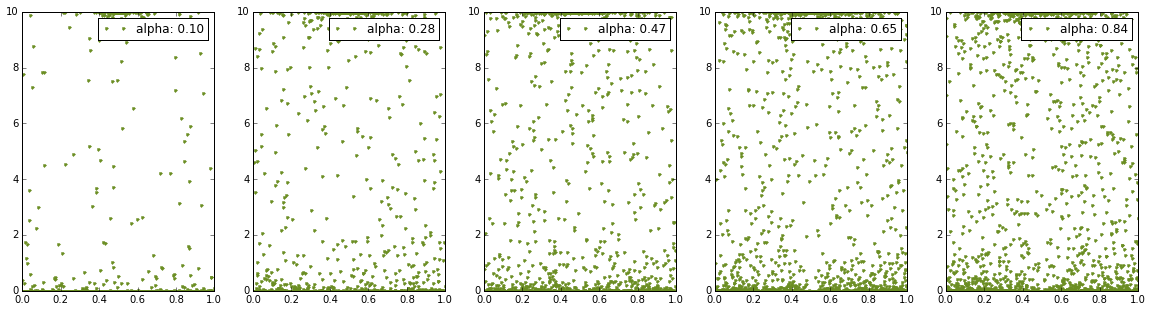
\includegraphics[width=\textwidth]{graphs/distribution1.png}
			\caption{Mass vs prediction}
		\end{subfigure}
		\begin{subfigure}[b]{0.95\textwidth}
			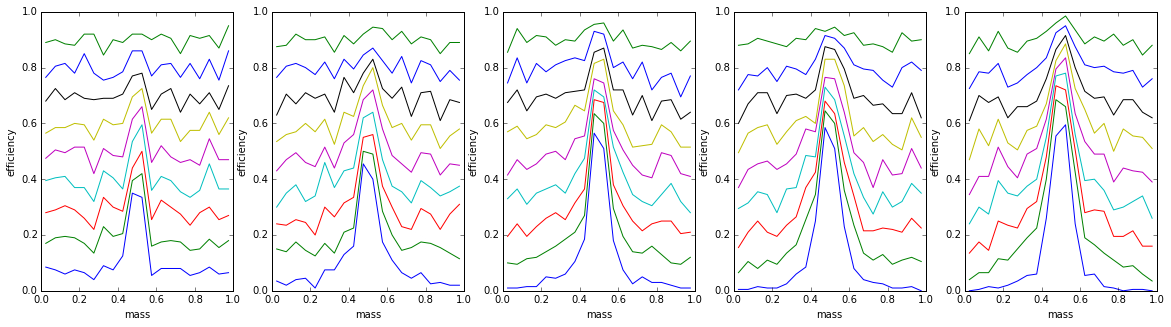
\includegraphics[width=\textwidth]{graphs/efficiencies1.png}
			\caption{Efficiencies}
		\end{subfigure}
		\caption{Peak distribution}
\end{figure}

\begin{figure}[H]
\centering
	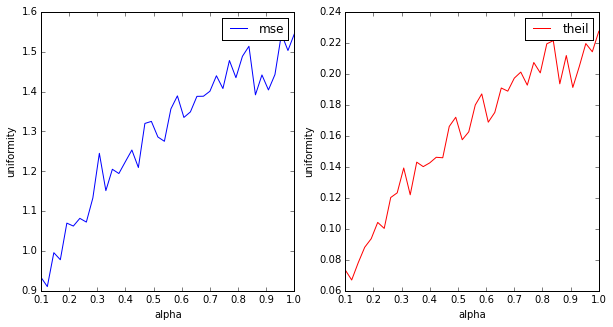
\includegraphics[width=8cm]{graphs/measures1.png}
	\caption{SDE and Theil}
\end{figure}

\begin{figure}[H]
\centering
		\begin{subfigure}[b]{0.95\textwidth}
			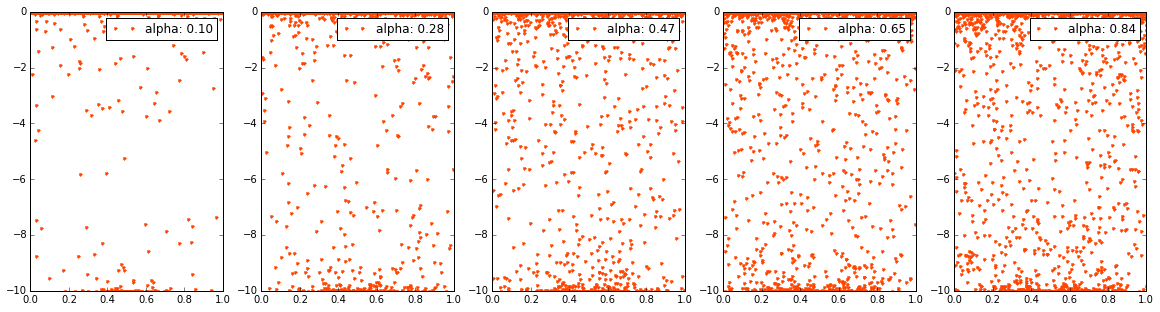
\includegraphics[width=\textwidth]{graphs/distribution2.png}
			\caption{Mass vs prediction}
		\end{subfigure}
		\begin{subfigure}[b]{0.95\textwidth}
			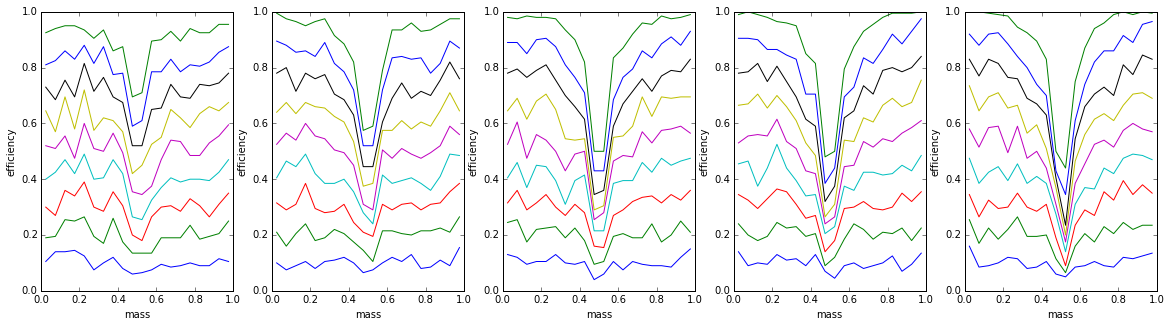
\includegraphics[width=\textwidth]{graphs/efficiencies2.png}
			\caption{Efficiencies}
		\end{subfigure}
		\caption{Pit distribution}
\end{figure}

\begin{figure}[H]
\centering
	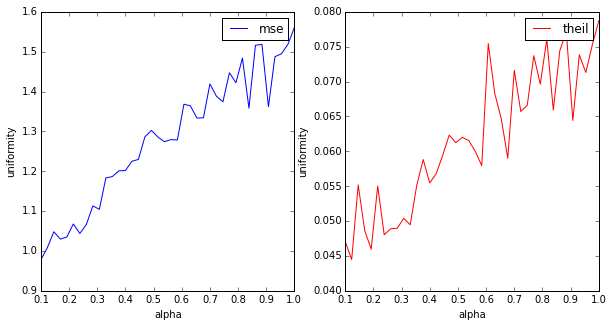
\includegraphics[width=8cm]{graphs/measures2.png}
	\caption{SDE and Theil}
\end{figure}

From these figures we can see that SDE has the same value and it is not able to make difference between these distributions, while Theil can detect
these changes which are in the acordance with the very purpose of Theil measure.